\chapter[SM SysId of LTI systems with EIV noise structure]{Set-Membership SysId of LTI systems with Errors-In-Variables (EIV) noise structure}

We have seen in the last chapter that an equation-error noise structure leads to a solution of LP problems for obtaining the Parameter Uncertainty Intervals, however, we have seen that there are some drawbacks. 
First of all the way we can find a bound $\Delta_e$ on the noise samples.
Then, the objective here is to find a way for dealing with the 'original' problem, that is the one using the output and input samples corrupted by noise.

\section{ Feasible Parameter Set in the EIV set-up}
In order to define also for this type of set-up the feasible parameter set, we have to follow the same road as we have done before. In particular we have to put together:
\begin{description}
    \itemsep-0.2em
    \item[A-priori information on the system] We know that the system belongs to a certain class $\mathcal{F}$, moreover we know the order $n$ of the system itself.
    \item[A-priori information on the noise] In particular the way the uncertainty enters the identification problem (we assume here the most general case when both input and output are corrupted by noise) and the boundedness of the noise samples, in particular
    \begin{equation}
        \vert \eta(k) \vert \le \Delta_\eta \quad
        \vert \xi(k) \vert \le \Delta_\xi
        \quad
        \forall k=1,...,N
    \end{equation}
    \item[A-posteriori information] They are nothing but the experimentally collected data $$\tilde{y}(k)=y(k)+\eta(k), \quad 
    \tilde{u}(k)=u(k)+\xi(k) $$
\end{description}
For an \textbf{LTI system of order $n$} the feasible parameter set is defined as follows: 

\begin{equation}\label{eq:FPS}
    \begin{aligned}
        \mathcal{D}_\theta = \{
            &\theta\in\mathbb{R}^p:  
            (\tilde{y}(k)-\eta(k))+\sum_{i=1}^n{\theta_i}\ ({y}(k-i)-\eta(k-i))=\\
            &\sum_{j=0}^m \theta_j \ (u(k-j)-\xi(k-j)), \quad
            k=n+1,...,N
        \} 
    \end{aligned}
\end{equation}
\noindent
In this context the definition of PUI is always the same, and the extrema of such an interval are defined as before by  solving the optimization problems:

\begin{equation*}
    \underline{\theta}_j = \min_{\theta\in\mathcal{D}_\theta} \theta_j, \quad 
    \overline{\theta}_j = \max_{\theta\in\mathcal{D}_\theta} \theta_j
    \Longrightarrow PUI_{\theta_j}=[\underline{\theta}_j,\overline{\theta}_j]
\end{equation*}
At this point the question is: \textbf{what type of $\mathcal{D}_\theta$ I obtain?} 
\section{Extended Feasible Parameter Set $\mathcal{D}_{\theta,\eta,\xi}$}
How we are able to see in the (\ref{eq:FPS}) the set definition depends also on the noise samples. The difference here is that I cannot eliminate them without adding any approximation. Substancially, I am introducing a non trivial number of new unknown in the description of the set: for $N$ collected samples, $2N$ new variables are added, which cannot be eliminated. For this reason we have to \textit{enlarge} the set $\mathcal{D}_\theta$ involving also the new variables. In this way we introduce the so-called \textbf{Extended Feasible Parameter Set (EFPS)} which we indicate with $\mathcal{D}_{\theta,\eta,\xi}$. \\
In order to better understand this aspect, let us consider a toy-example in which we have a single parameter $\eta(1)$ which is added to the pair $\theta_1, \theta_2$. The EFPS in this case -- how the figure below shows -- is a subset of $\mathbb{R}^3$.
\vspace{-0.2cm}
\begin{figure}[h]
    \centering
    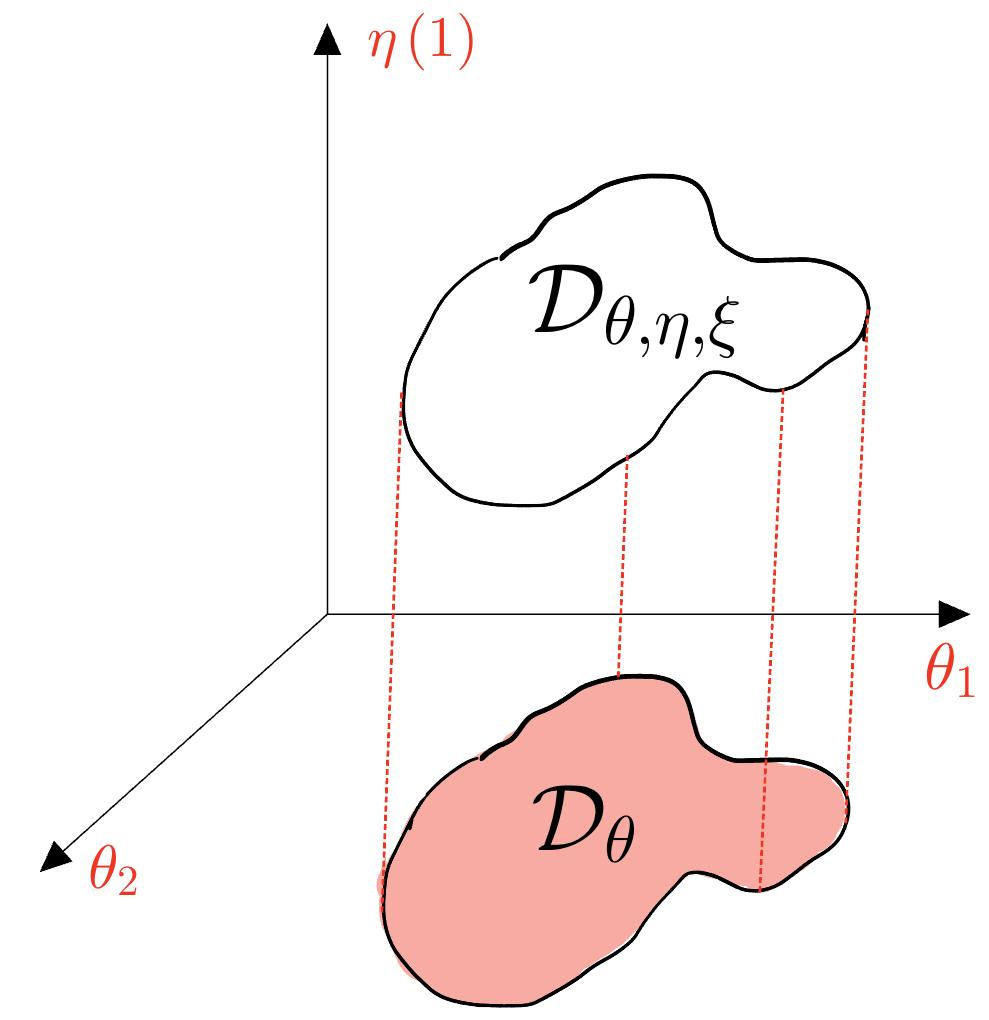
\includegraphics[scale=0.15]{img/EFPS.jpeg}
    \caption{Example in $\mathbb{R}^3$ of the Extended feasible parameter set}
\end{figure}

\noindent
The FPS $\mathcal{D}_\theta$ is nothing but the projection on the $(\theta_1,\theta_2)$ plane of the set $\mathcal{D}_{\theta,\eta}$, in this case no parameter $\xi$ is present.

\noindent
The definition of the \textbf{Extended Feasible Parameter Set} becomes the following:
\begin{equation}
    \begin{aligned}
        \mathcal{D}_{\theta,\eta,\xi} = \{
            &\theta\in\mathbb{R}^p, \eta\in\mathbb{R}^N, \xi \in \mathbb{R}^N: 
            \tilde{y}(k)-\eta(k) + \theta_1 (y(k-1)-\eta(k-1)) +\\
            &+\theta_2 (y(k-2)-\eta(k-2))+\dots+\theta_n (y(k-n)-\eta(k-n))=\\
            &=\theta_{n+1} (u(k)-\xi(k))+\theta_{n+2} (u(k-1)-\xi(k-1)) + ...+\\
            &\theta_{n+m+1} (u(k-m)-\xi(k-m)), \quad k=n+1,...,N\\
             &\vert \xi(k) \vert \le \Delta_\xi, \quad 
            \vert \eta(k) \vert \le \Delta_\eta, \quad k=1,...,N
        \}
    \end{aligned}
\end{equation}

\noindent
Such a set is defined by \textbf{nonlinear} and \textbf{non-convex} constraints and then the set is non-convex. In the specific case, the constraints that arises are \textbf{bilinear ones} which are a particular class of \textbf{polynomial constraints}. In general we know that is very hard to obtain a global minimum from a non-convex optimization problem, in this case using some tools for \textit{polynomial optimization} it is possible to reach a global minimum.\\

\noindent
In this framework the problem of finding the PUIs becomes:
{\large{
    \begin{equation}
        PUI_{\theta_j} = [\underline{\theta}_j,\overline{\theta}_j] \Longrightarrow 
        \underline{\theta}_j = \min_{\theta\in\mathcal{D}_{\theta,\eta,\xi} } \theta_j,    \quad
        \overline{\theta}_j = \max_{\theta\in\mathcal{D}_{\theta,\eta,\xi}} \theta_j
    \end{equation}
}}


 


